\documentclass[tikz,border=5pt]{standalone}
\usepackage{tikz}
\usepackage{pgfplots}
\pgfplotsset{compat=1.18}

\begin{document}

% Double-Barrier Resonance Structure
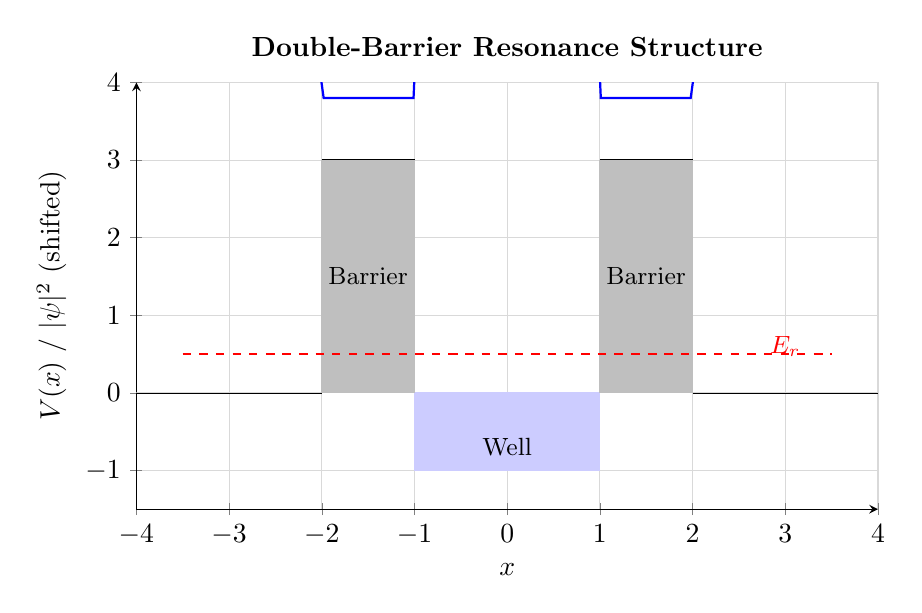
\begin{tikzpicture}
\begin{axis}[
    width=11cm,
    height=7cm,
    xlabel={$x$},
    ylabel={$V(x)$ / $|\psi|^2$ (shifted)},
    title={\textbf{Double-Barrier Resonance Structure}},
    xmin=-4, xmax=4,
    ymin=-1.5, ymax=4,
    axis lines=left,
    grid=major,
    grid style={gray!30},
    samples=200,
]

% Potential function
\addplot[thick,black,domain=-4:-2] {0};
\addplot[thick,black,domain=-2:-1] {3};
\addplot[thick,black,domain=-1:1] {-1};
\addplot[thick,black,domain=1:2] {3};
\addplot[thick,black,domain=2:4] {0};

% Fill regions
\addplot[gray!30,fill=gray!30,domain=-4:4] {0} \closedcycle;
\addplot[blue!20,fill=blue!20,domain=-1:1] {-1} \closedcycle;
\addplot[gray!50,fill=gray!50,domain=-2:-1] {3} \closedcycle;
\addplot[gray!50,fill=gray!50,domain=1:2] {3} \closedcycle;

% Resonance level
\addplot[red,dashed,domain=-3.5:3.5] {0.5};
\node[red,font=\small] at (axis cs:3,0.6) {$E_r$};

% Wave function amplitude (sketch)
\addplot[blue,thick,samples=100,domain=-4:4] 
    {3.5 + (abs(x)<1 ? 2.5 : (abs(x)<2 ? 0.3 : 1))};
\node[blue,font=\small] at (axis cs:3,4.2) {$|\psi|^2$};

% Labels
\node[font=\small] at (axis cs:0,-0.7) {Well};
\node[font=\small] at (axis cs:-1.5,1.5) {Barrier};
\node[font=\small] at (axis cs:1.5,1.5) {Barrier};

\end{axis}
\end{tikzpicture}

\end{document}
